\documentclass[noauthor,nooutcomes,12pt]{ximera}

\graphicspath{  
{./}
{./whoAreYou/}
{./drawingWithTheTurtle/}
{./bisectionMethod/}
{./circles/}
{./anglesAndRightTriangles/}
{./lawOfSines/}
{./lawOfCosines/}
{./plotter/}
{./staircases/}
{./pitch/}
{./qualityControl/}
{./symmetry/}
{./nGonBlock/}
}


%% page layout
\usepackage[cm,headings]{fullpage}
\raggedright
\setlength\headheight{13.6pt}


%% fonts
\usepackage{euler}

\usepackage{FiraMono}
\renewcommand\familydefault{\ttdefault} 
\usepackage[defaultmathsizes]{mathastext}
\usepackage[htt]{hyphenat}

\usepackage[T1]{fontenc}
\usepackage[scaled=1]{FiraSans}

%\usepackage{wedn}
\usepackage{pbsi} %% Answer font


\usepackage{cancel} %% strike through in pitch/pitch.tex


%% \usepackage{ulem} %% 
%% \renewcommand{\ULthickness}{2pt}% changes underline thickness

\tikzset{>=stealth}

\usepackage{adjustbox}

\setcounter{titlenumber}{-1}

%% journal style
\makeatletter
\newcommand\journalstyle{%
  \def\activitystyle{activity-chapter}
  \def\maketitle{%
    \addtocounter{titlenumber}{1}%
                {\flushleft\small\sffamily\bfseries\@pretitle\par\vspace{-1.5em}}%
                {\flushleft\LARGE\sffamily\bfseries\thetitlenumber\hspace{1em}\@title \par }%
                {\vskip .6em\noindent\textit\theabstract\setcounter{question}{0}\setcounter{sectiontitlenumber}{0}}%
                    \par\vspace{2em}
                    \phantomsection\addcontentsline{toc}{section}{\thetitlenumber\hspace{1em}\textbf{\@title}}%
                     }}
\makeatother



%% thm like environments
\let\question\relax
\let\endquestion\relax

\newtheoremstyle{QuestionStyle}{\topsep}{\topsep}%%% space between body and thm
		{}                      %%% Thm body font
		{}                              %%% Indent amount (empty = no indent)
		{\bfseries}            %%% Thm head font
		{)}                              %%% Punctuation after thm head
		{ }                           %%% Space after thm head
		{\thmnumber{#2}\thmnote{ \bfseries(#3)}}%%% Thm head spec
\theoremstyle{QuestionStyle}
\newtheorem{question}{}



\let\freeResponse\relax
\let\endfreeResponse\relax

%% \newtheoremstyle{ResponseStyle}{\topsep}{\topsep}%%% space between body and thm
%% 		{\wedn\bfseries}                      %%% Thm body font
%% 		{}                              %%% Indent amount (empty = no indent)
%% 		{\wedn\bfseries}            %%% Thm head font
%% 		{}                              %%% Punctuation after thm head
%% 		{3ex}                           %%% Space after thm head
%% 		{\underline{\underline{\thmname{#1}}}}%%% Thm head spec
%% \theoremstyle{ResponseStyle}

\usepackage[tikz]{mdframed}
\mdfdefinestyle{ResponseStyle}{leftmargin=1cm,linecolor=black,roundcorner=5pt,
, font=\bsifamily,}%font=\wedn\bfseries\upshape,}


\ifhandout
\NewEnviron{freeResponse}{}
\else
%\newtheorem{freeResponse}{Response:}
\newenvironment{freeResponse}{\begin{mdframed}[style=ResponseStyle]}{\end{mdframed}}
\fi



%% attempting to automate outcomes.

%% \newwrite\outcomefile
%%   \immediate\openout\outcomefile=\jobname.oc
%% \renewcommand{\outcome}[1]{\edef\theoutcomes{\theoutcomes #1~}%
%% \immediate\write\outcomefile{\unexpanded{\outcome}{#1}}}

%% \newcommand{\outcomelist}{\begin{itemize}\theoutcomes\end{itemize}}

%% \NewEnviron{listOutcomes}{\small\sffamily
%% After answering the following questions, students should be able to:
%% \begin{itemize}
%% \BODY
%% \end{itemize}
%% }
\usepackage[tikz]{mdframed}
\mdfdefinestyle{OutcomeStyle}{leftmargin=2cm,rightmargin=2cm,linecolor=black,roundcorner=5pt,
, font=\small\sffamily,}%font=\wedn\bfseries\upshape,}
\newenvironment{listOutcomes}{\begin{mdframed}[style=OutcomeStyle]After answering the following questions, students should be able to:\begin{itemize}}{\end{itemize}\end{mdframed}}



%% my commands

\newcommand{\snap}{{\bfseries\itshape\textsf{Snap!}}}
\newcommand{\flavor}{\link[\snap]{https://snap.berkeley.edu/}}
\newcommand{\mooculus}{\textsf{\textbf{MOOC}\textnormal{\textsf{ULUS}}}}


\usepackage{tkz-euclide}
\tikzstyle geometryDiagrams=[rounded corners=.5pt,ultra thick,color=black]
\colorlet{penColor}{black} % Color of a curve in a plot



\ifhandout\newcommand{\mynewpage}{\newpage}\else\newcommand{\mynewpage}{}\fi

\usepackage{fullpage}
\makeatletter
%% no number for activity
\newcommand\logostyle{%
  \def\activitystyle{activity-chapter}
  \def\maketitle{%
                {\flushleft\small\sffamily\bfseries\@pretitle\par\vspace{-1.5em}}%
                {\flushleft\LARGE\sffamily\bfseries\@title \par }%
                {\vskip .6em\noindent\textit\theabstract\setcounter{problem}{0}\setcounter{sectiontitlenumber}{0}}%
                    \par\vspace{2em}
                    \phantomsection\addcontentsline{toc}{section}{\textbf{\@title}}%
                     \setcounter{titlenumber}{0}}}
\makeatother
\newcommand{\nameblankgen}{\noindent\textbf{Name(s) (please print):}\ \hrulefill \\

\hrulefill}
\logostyle



\title{Repeating steps}
\author{Bart Snapp}

\begin{document}
\begin{abstract}
  Don't type so much, let the turtle repeat!
\end{abstract}
\maketitle

\nameblankgen

\begin{multicols*}{2}
  Drawing pictures in \LOGO\ often means making the turtle do things
  over and over again. The drawing-turtle doesn't mind, but there are
  efficient ways to communicate. One way is the \lc{repeat} command.
\begin{logo}
repeat 4 [
  fd 100
  lt 90
  ]
\end{logo}

Which produces a square. We can name this procedure \lc{square} (or
\lc{susan} or \lc{bob}) by using \lc{to} \dots \lc{end}:

\begin{logo}
to square
  repeat 4 [ fd 100 lt 90 ]
end
\end{logo}
Now the code above draws NOTHING. To make it draw something, add the command \lc{square} at the end:
\begin{logo}
to square
  repeat 4 [ fd 100 lt 90 ]
end
square  
\end{logo}
This draws:
\begin{logoout}
\begin{tikzpicture}[turtle/distance=2cm]
  \draw [thick,black,turtle={home,forward,left,forward,left,forward,left,forward}];
  \node at (0,0) {\turtle};
\end{tikzpicture}
\end{logoout}

Now that we have \lc{square} around, we can repeat it too! We'll draw a flower:

\begin{logo}
ht setcolor 1 fill 
setwidth 20 setcolor 2
bk 300
setwidth 100
lt 90 
fd 800
pu home pd
setwidth 10 setcolor 6-random 4
repeat 12 [square rt 30]
\end{logo}
\begin{logoout}
    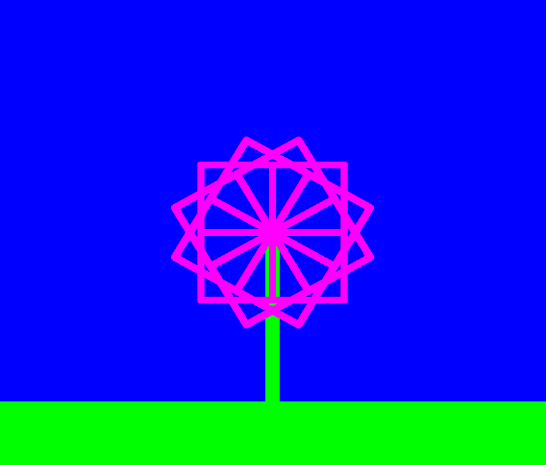
\includegraphics[width=.3\textwidth]{flower.png}
\end{logoout}

Let's make field of flowers!

\section{Commands to know}
\begin{tabular}{lll}
  \lc{CMD}   & Description                 \\ \hlinewd{1pt}
  \lc{repeat \# [ BODY ]} & \lc{BODY} repeats \lc{\#} times  \\
  \lc{to NAME BODY end}   & a new command \lc{NAME}\\
  \lc{setcolor \#}   & set the color to \lc{\#} \\
  \lc{fill} & bucket fill \\ 
  \lc{setwidth \#}   & set pen width \lc{\#}\\
  \lc{random \#}     & \begin{minipage}[t]{2in}random number between $0$ and $\lc{\#} -1$\end{minipage}
\end{tabular}


\end{multicols*}

\newpage

\begin{problem}
  Above, there is code that draws a flower. Explain in words what each
  line of the code does.
\end{problem}

\newpage

\begin{problem}
  Make a command \lc{flower} that will make a small version ($\sim 50$
  units tall) of the flower above.  Show your code and your picture.
\end{problem}

\newpage


\begin{problem}
  What direction is the turtle facing after your flower command is
  made? Explain how you know with words/pictures.
\end{problem}

\newpage

\begin{problem}
  Make a command \lc{patch} that will make a `patch' of three flowers
  in a row.  Show your code and your picture. 
\end{problem}

\newpage

\begin{problem}
  Make a command \lc{field} that will produce a field of color
  \lc{[80 100 80]} covered in patches of flowers. Show your
  code and your picture.
\end{problem}


\end{document}
